%% This is an example first chapter.  You should put chapter/appendix that you
%% write into a separate file, and add a line \include{yourfilename} to
%% main.tex, where `yourfilename.tex' is the name of the chapter/appendix file.
%% You can process specific files by typing their names in at the 
%% \files=
%% prompt when you run the file main.tex through LaTeX.




\chapter{Introduction}



% copy-paste
% The architecture of deep convolutional neutral networks (CNNs) has evolved for years, becoming more accurate and faster. Since the milestone work of AlexNet [1],
% the ImageNet classification accuracy has been significantly improved by novel structures, including VGG [2], GoogLeNet [3], ResNet [4,5], DenseNet [6], ResNeXt [7], SE-Net [8], and automatic neutral architecture search [9,10,11], to name a few.

Since the introduction of the milestone work of AlexNet \cite{alexnet??} the architecture of deep convolutional neutral networks (CNNs) has been constantly evolving over the years, becoming more accurate and faster. 

Many studies have focused on designign new architectures to increase accuracy for image classification on Imagnet without considering speed of the models, but real-world systems often require high recognition accuracy with low latency.

There are papers which focus on imroving speed by reducing number of computations inside network or by minimizing number of parameters used. In Chapter 2 we discuss why such optimization don't always result in low inference speed on real-life accelerators.


In Chapter 3 we discuss recent modifications for training recipes and minor changes to architectures which improve model performance without compromising speed

In Chapter 4 we propose a novel desing choice not discussed in the literature before which is one of main points of this paper

In Chapter 5 we show result of out experiments which try to balance on speed-accuracy tradeoff by applying only changes that have minor impact on speed. By combining multple minor changes we obtain close to SOTA performance on large-scale image recogntiong dataset ImageNet. 


не могу писать на английском, потому что постоянно отвлекаюсь и пытаюсь копировать, а нужно изливать свои мысли, так будет быстрее (((




Something goes here

intro is close to \cite{lin2020neural_genet} & \cite{ridnik2021_tresnet}

О чём блять вообще диплом? хочу быструю и одновременно качественную сетку. 
Многие работы принимают во внимание только качество, но для практических применений очень важна именно скорость, поэтому мы хотим постоянно иметь её во внимание. Есть много разных акслелераторов (см. отдельную главу о них), но эта работа фокусируется исключительно на современных видеокартах. Полученные выводы могут не выполняться для мобильных платформ (тут ссылочки на работы об этом). 


\chapter{Chapter2 (Speed)}


% bottlenecks induced by FLOPs oriented optimizations - говорю о том, что определине "маленькая" сеть и "быстрая" сеть неоднозначны. можно смотреть на параметры, можно на FLOPS, можно на MAC, можно на real-life performance. ссылаюсь на работы которые показывают что связь между FLOPS | params | mac и скоростью нифига не линейная. можно вставить графики сравения по FLOPS похожие на те что в \cite{ma2018shufflenetv2}

\section{Intro (again)}

Real world tasks often have computational constarains on the design of arcitecures. Design of light-weight models with good speed-accuracy tradeoffs has been explored extensively before \cite{howard2017mobilenetv1} \cite{mobilenetv2} \cite{ma2018shufflenetv2} \cite{zhang2018shufflenet}.  % \cite{Xception} 

To measure complexity of the model some works use number of computations it does. Examples of such metrics are floating point operations (FLOPs) and multiply-accumulate operations (MACCs). Other focus on minimizing of number of trainable parameters. This metrics are indirect approximation of direct metric such as speed or latency. Previous works has shown \cite{design_spaces} that factors affecting inference latency on modern accelerators are complicated and direct measurement on target device should be preffered. (тут можно еще цитирований из \cite{ma2018shufflenetv2} p.2 набрать).

The deep learning models could be run on CPU or on a number of other accelerators. Most popular ones being GPUs (graphic processing units) and TPUs (Tensor processing units), ... (тут примеры других ускорителей). (тут статистика по использованию акслелераторов)

This works focuses on optimizing and developing networks specially optimized for **modern GPUs**, such narrow focus allows to better utilize the knoledge about what constrains speed the most. Obtained results may not be applicable if models have to be run on CPUs or mobile devices (тут можно что-то из Effnet lite процитировать)

% \cite In-datacenter performance analysis of tensor processing units
% \cite The deep learning revolution and its implication for computer architecture and chop desin

\section{Definitions}

"It’s dot products all the way down" 

Many of the computations inside neural networks are dot products like this: $y = w[0]*x[0] + w[1]*x[1] + \cdots \ldots w[n] * x[n]$ where $w$ and $x$ are two vectors and $y$ is a scalar. There are two main ways to calculate number of computations in such operation. First is to count $ w[0] * x[0] + \cdot $ as one multiply-accumulate or 1 MACC. The __accumulation__ operation here is addition. In the example above we have $n$ MACCs. 


NOTE: 
Technically speaking there are only n - 1 additions in the example above. Think of MACCs as being an approximation, simular to Big-O notation used in approximation of algorithm complexity.

Second is to count number of direct floating point operations (FLOPs), in the example above there are $2n - 1$ FLOPs, since there are n multiplications and n additions. FLOPs should not be confused with floating point operations per second (FLOPS) used to measure hardware performance. Because matrix-multiplications is the core operation in neural networks, many modern accelerators have special multiply-and-accumulate units, called tensor cores 
% \cite Volte: performance and programmability 
in GPUs and matrix multply units in TPUs % \cite two papers from comments above [30] [14] in Searching ....
This means that 1 MACC could be perfomed usign 1 instruction, so in this work definition of FLOPs follows \cite{zhang2018shufflenet}, i.e. number of multiply-adds. Making FLOPs and MACC interchangeble.

Another important property of the netork is dynamic random-access memory(DRAM) traffic for read and write of model parameters, activations and intermidiate feature maps. Measuring exact number of DRAM read/write bytes could be complicated and requires special software. DRAM could be approximated by memory footprints of input and output tensors. This metric is called Convolutional Input/Output (CIO) ( cite HardNet ) and is proportional to to the real DRAM traffic measurement. For a typical convolution kernel with $c$ channels, width $w$ and height $h$ CIO could be calculated using eq ??

$$
C I O=\sum_{l}\left(c_{i n}^{(l)} \times w_{i n}^{(l)} \times h_{i n}^{(l)}+c_{o u t}^{(l)} \times w_{o u t}^{(l)} \times h_{o u t}^{(l)}\right)
$$



\section{Why FLOPs and latency do not correlate}

We reasonably assume that model speed is either compute-bound or memory-(bandwidth)-bound as they don't fit in on-chip memories. DRAM access can dominate system inference time due to limited memory bandwidth. An ML model can achieve peak FLOPs/sec and fully utilize accelerators only when its operational density, which is MACs over CIO (MoC) is sufficiently large (and is enough to saturate accelerators performance ?? need to clarify __saturate__). 

(вотвну сюда, потом разберусь в compunding тоже говорил что не наблюдают связи между FLOPS и скоростью. может надо воткнуть это как рефернс куда-то)
%% maybe need to move MoC into definition??
%% also later I use a slightly different MoC which also accouts for number of parameters accesses. Need to modify definition here, or use true MoC in later chapter

From that we can see why minimizing number of FLOPs don't always correlate with latency, such minization is only reasonable when we are compute-bounded in this layer. 

Several papers has observed this lack of correlation and proposed several key principles for desingin high speed models specifically on GPUs (cite something). Rather than providing them as is we will validate each claim with a set of experiments to observe the switch between compute-bound/memory-bound regions directly.

\subsection{Depthwise Separable Convolutions}

Depth-wise convolutions (DW conv in short) have been proposed as an efficient alternative to traditional 2d convolutions. In the regular 2d convolution the filter is as deep as the input and lets us freely mix channels to generate each element in the output. In Depthwise convolutino each channel is kept separate. 

Mixing channels is important for  neural networks, so the depthwise is more commonly used in combination with an additional step to mix the channels (pointwise convolution), such operation is called depthwise-separable convolution. See \ref{convs} for visual explanation of difference between conv and DepSep conv. 

\begin{figure}[h]
    \centering
         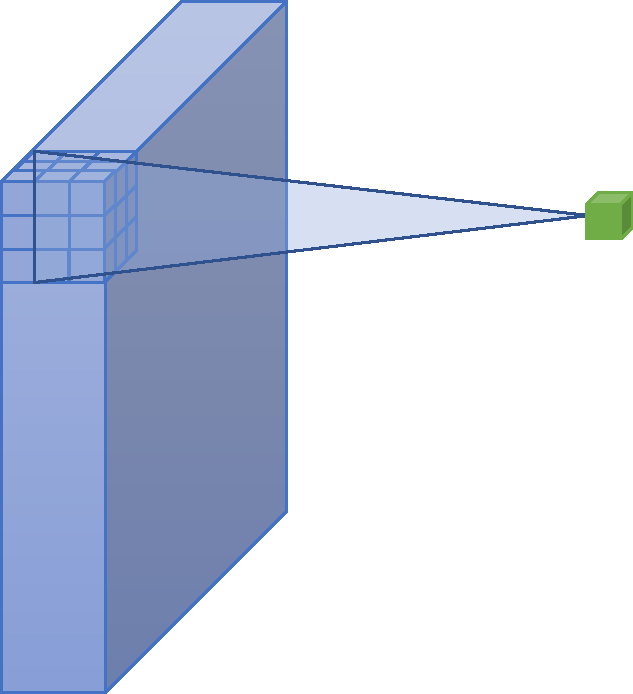
\includegraphics[width=0.13\textwidth]{images/conv.pdf}
         \hfil
         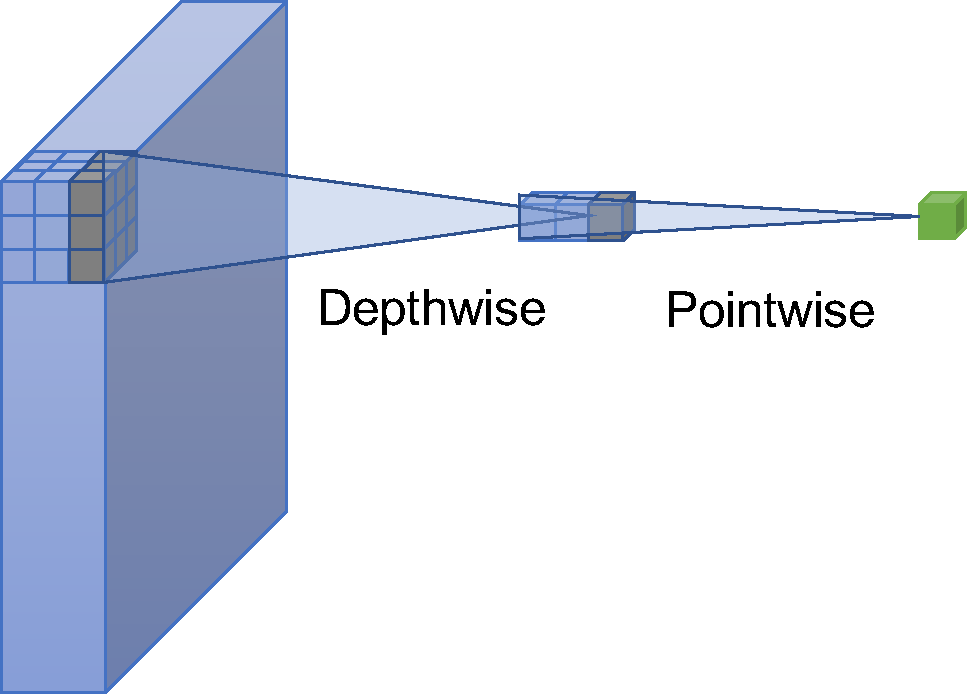
\includegraphics[width=0.2\textwidth]{images/conv_DepSep.pdf}
    \caption{Standard convolution and depthwise separable convolution.}   \label{fig: convs}
    \end{figure}


DepSep convolutions are used in models such as (cite excpetion mobilenet effnet) and more. They have less parameters and require less floating point operations (FLOPs) to compute, however as we mentioned above metrics such as FLOPs and parameter sizes may not correspond with real-world performance. Let $C_{in}, C_{out}, H, W$ be number of input/output channels, feature width and height. We will only discuss case of convlution with squre kernel size $K$. To make comparison easier we will use following paramters: $K=3$, $H=W=224$, $C_{in} = C_{out}=128$, representing a typcial convolution inside a typical ResNet-like model.  

Usual convolution has: $ K \times K \times C_{in} \times C_{out} \approx 147k$ parameters, and $ K \times K \times C_{in} \times C_{out} \times H \times W \approx 7.4 GFLOPs$. Depthwise separable convolution has: $ K \times K \times C_{in} + C_{in} \times C_{out} \approx 18k$ parameters and $ K \times K \times C_{in} \times H \times W + C_{in} \times C_{out} \times H \times W \approx 0.88$ GFLOPs. We can see that typical DepSep convolution has ten times less parameters and FLOPs. Empirical benchmarks % cite https://tlkh.dev/depsep-convs-perf-investigations/
(maybe need more details about software and hardware - TF 2.1, CUDA 10.1, cuDNN 7.6.5, or can simple leave it inside reference??)

% this table is generated using my code on PyTorch 1.7.1 + CUDA 10.2. Numbers are slightyl different but the conclusino is the same
% [ Stem conv. Shape: torch.Size([32, 128, 224, 224]) ]
% |  description
% 16 threads: ----------------------------------
%       Reg Conv. Params: 147.5k  |     214.2
%       Conv DW. Params: 1.2k     |      43.3
%       Conv Sep. Params: 17.5k   |      88.9
% 4670, 23150, 11235 convs / sec
% 7.4 GFLOPs, 57.8 MFLOPs, 0.88 GFLOPs
% reg conv flops / dw conv flops ~= 128
% 34.5 TFLOPS, 1.33 TFLOPS, 9.9 TFLOPS (8 in fp32)
% 
% Times are in microseconds (us).
% same as above but in fp32
% 16 threads: ----------------------------------
%       Reg Conv. Params: 147.5k  |     488.2
%       Conv DW. Params: 1.2k     |     119.4
%       Conv Sep. Params: 17.5k   |     243.6

% [ Middle conv. Shape: torch.Size([32, 1024, 32, 32]) ]
%                                  |  description
% 16 threads: -----------------------------------
%       Reg Conv. Params: 9437.2k  |     225.0
%       Conv DW. Params: 9.2k      |       7.4
%       Conv Sep. Params: 1057.8k  |      37.2
% 
% 9.7 GFLOPs, 9.43 MFLOPs, 1 GFLOPs
% reg conv flops / dw conv flops ~= 1028
% 43.1 TFLOPS, 29.1 TFLOPS
% Times are in microseconds (us).
% IMPROTANT CONCLUSION. While DW is always much slower than regular, on deeper feature maps it significantly reduces number of FLOPs
% making it anyway better. On my GPU the  

show that regular convolutions achieve up to 30.3 TFLOP/sec, while DepSep convolutions only achieve 3.8 TFLOP/sec. We can see that despite much lower number of FLOPs, DepSep convolutions are much worse in utilizing modern accelerator. To prove that in this case we're memory-bounded, let's compute arithmetic intesity (MoC) to better undestand computational profile of each convolution. We naively estimate memeory access to be sum of number of parameters and number of activations, this assumtion will give us a lower bound, when no redundant memory accesses are performed. 

Usual convolution has: $ N_{parameters} + N_{activations} = K \times K \times C_{in} \times C_{out} + (C_{in} + C_{out}) \times H \times W \approx 26.0$ MB of memory accesses. Depthwise separable convolution has: $ N_{parameters} + N_{activations} = K \times K \times C_{in} + C_{in} \times C_{out} + (C_{in} + C_{out}) \times H \times W \approx 25.7$ MB of memory accesses. Then MoC is 569.5 and 68.4 for regular and DepSep convolution respectively. We immediately see that, normal convolutions have almost ten times as much arithmetic intensity compared to DepSep convolutions, is much lower to compute-bound than to memory-bound effectively utilizing accelerator. 

The conclusion from above analysis is that DepSep convolutions are only efficient when computing them is not memory-bounded. This is true in deeper layers of ResNet-like models where spatial size is reduced and number of feature maps is increased. 

\subsection{Pointwise convolutions}

Pointwise convolution is a 2d convolution with kernel size being 1x1, they are also referenced as conv1x1 later in this section. This type of convolutions is used intensively in Bottleneck of ResNet50 model and in almost every model after that (cite ... as many papers as we want). Pointwise convolution most often are used to increase/decrese number of channels (cite ResNet again) or to mix information betwenn channels after Depthwise convolution. While conv1x1 are cheap in terms of FLOPs the have very almost the same CIO as regular 3x3 convolutin which means they may become memory-bottlenecks. This type of convolutinos may also become memory-bounded when ratio of number of input channels to output channels is large. Both this properties could be investigated (ужасно написано кмк).

In fig ?? (график с MACs over CIO похожий на график из HardNet) you can see 
(тут порассуждать о том, что conv1x1 недоутилизируют аккселератор, потому что вычислений маловато. единственное )

We can perform analysis of MoC simular to the previous chapter. We will compare achieved FLOPS when we apply conv1x1 in the beginning of the network and when we apply them in the deeper layers. Let $C_{in}, C_{out}, H, W$ be number of input/output channels, feature width and height. Kernel size $K$ is 1. First case: $H=W=224, C_{in} = 16, C_{out}=128$, Second case: $H=W=32, C_{in} = C_{out}=1024$, representing a typcial conv1x1 at the beginning and in the deeper layers of a typcial ResNet-like model.

**(need better naming than __first__ and __second__)**

First conv has $ 1 \times 1 \times C_{in} \times C_{out} \approx 2k$ parameters. And $ 1 \times 1 \times C_{in} \times C_{out} \times H \times W \approx 0.1 $ GFLOPs

Second conv has \approx 1M parameters and \approx 1 GFLOPs. 

% speed using half on V100, Pytorch 1.7.1, CUDA 10.1
% stem convs ~= 27 microseconds / conv = 37000 convs / sec ~= 3.7 TFLOPS
% deepre convs ~= 29 microseconds / conv = 34500 convs / sec ~= 34 TFLOPS
%

Empirical benchmarks show that first conv achieves \approx 3.7 TFLOP/sec, while conv1x1 in deeper layer (second conv) achieves \approx 34 TFLOP/sec. We can see a simular to DepSep conv pattern. Some conv1x1 give almost ten times lower accelerator utilization. Lets show that it again happens due to memory-bound.

(тут анализ по памяти)

(сюда нужно добавить рассчеты из HardNet что лучше использвовать одинаковок количество каналов, чем разное, потому что при одном и том же CIO это даёт разную плотность )

The conclusion from above analysis is that avoiding pointwise convolutions at the beginning of the network could help to avoid memory-bottleneck and increase speed of the model. This idea has been implicitly used in \cite{ridnik2021_tresnet} paper, where authors replaced pointwise convolutions in first blocks of the network with 3x3 convoultions which increased computation density and speed up the model, maintaining the same number of parameters. Authors did not provide any analysis about why it works, like i did (ужасно написано, нужно переписать. идея в том что авторы использоваил этот дизайн принцип, не понимая реально почему он работает, а мы тип объясняем прошлые статьи, через четкий анализ, что эмпирическеи подтверждает что мы правы)


(еще была статья про \cite{zhou2020_rethinking} где авторы вроде чето такое же предалагали??)

\subsection{Conclusion}


(это еще сырой кусок, потом перепишу)

* Due to use of matrix-multiply-and-accumulate units compute is significantly cheaper that on CPUs, resulting in ~35x higher TeraOps/sec of GPU v100 over typical CPU (cite something? can find in Searching for Fast Models)

* 

Empirical studies \cite{desing_spaces} has shown the factors affecting the inference latency on modern GPUs are rather complicated and is hard to predict directly. But at the same time following the principles mentioned below (above?) consistenly correlates with reduction in inference time. 
 

\subsection{Applying principle on practice}


Не могу определиться с порядоком. После рассуждений о структруе ограничений наврено нужно провести несколько экспериментов, а потом объеденить это в key principles, которые будут чем-то средним между принципами из HardNet, Searching.... и какими-то моими рассуждениями



\subsection{Examples of optimization}
Тут хочется привести пример Space2Depth модуля, который повышает эффективность за счет увеличения плотности операций в начале сети. 

 + тут можно написать про FusedConv который есть в EffNet v2, но появился вроде в EffNetX (??) 
% кусок нагло спизжен из Searching for Fast .... нужно будет переписать. 
еще про space2depth написано в статье \cite{ridnik2021_tresnet}


3.1. Efficient space-to-depth and space-to-batch
As pointed out in Section 2, convolutions need high parallelism in all dimensions (depth, batch, and spatial) to achieve high speed on TPUs and GPUs. However, insufficient parallelism because of the small depth and batch is the usual cause of low utilization and low performance on matrix units. We augment the search space with accelerator-friendly spaceto-depth and space-to-batch ops to increase depth and batch dimensions while keeping the total tensor volume the same. For space-to-depth ops, instead of using the memorycopy-reshape based ops provided by frameworks such as TensorFlow [6] and Pytorch [42], we customize an $n \times n$ convolution with stride-n to perform the space-to-depth operation, reshaping an $H \times W \times C$ tensor to an $H / n \times W / n \times C * n^{2}$ tensor. This approach has two advantages: 1) convolutions are much preferred by TPUs and GPUs because of their high operational intensity and execution efficiency; 2) in addition to reshaping the input tensor to improve operational intensity and efficiency, the $n \times n$ convolutions can also be trained


\chapter{Chapter3 Performance}

%%
нужно понять в каком порядке излагать мысль вообще. есть статьи, которые улучшают архитектуру, а есть которые предлагают новые способы обучения. проблема в том, что это не всегда разные статьи. новые блоки часто идут вместе с новыми трюками и сложно их разделить. (о чём пишут в compunding performance и гораздо более явно в resnet-RS). можно написать то же самое и скзаать что "я был первым" что на самом деле так, я об этом еще в начале прошлого года расговаривал). но мне для диплома нужно много текста, поэтому надо как-то завернуть рассжудения. как завернуть? 

разница между compunding и resnetRS в том, что первые бустят resnet без явного разделения что приходит от новых методов, а что приходит от изменения архитектуры, а RS явно показывает что приходит от архитектуры. 

%%

Models suitable for real-life deployment should be not only fast but also accurate. Definitonon of "accurate" differs in literature. In this paper we use top1 classification accuracy on imagenet as proxy for model performance on down-stream tasks. Section (???) discusses this choice in more details.


% at- tempts to combine existing techniques to create a practi- cal model are still uncommon

(нужно еще где-то сказать что со временем растет уровень того что такое бейзлайн. если в 2016м году резнет50 был 75.6, то сейчас если он ниже 79, то сравнение нечестное. самое честное что можно (и нужно делать) это использовать одинаковые трюки как во время обучения своей новой супер-пупер мега модели так и во время обучения старого-доброго резнета)

\subsection{Why Imagenet}

Imagenet Large Scale Vision Recognition Challenge also known as ILSVRC2012 or simply Imagenet is ..... (тут чутка про историю датасета и разер и наврено можно написать что это подмножество). ILSVRC2012 is the most used dataset in computer vision (cite something, maybe after MNIST and CIFAR). In recent years with models becoming larger and demanding more and more data, it became a de-facto stardart benchmark for any new architecture. Optimizing j

Since the breakthrought of AlexNet improving convolutional neural networks lead to improvements in other fields of computer vision. Typically researchers optimize models on classification problems using ImageNet (cite it) as proxy. It has been shown (where cite) than improvments from Imagenet do transfer to other domains.  

In this papepr we will use top1 1 classification accuracy on Imagenet as metric of model performance. 

Top-1 Thetop-1 is a measure of classification accuracy on the ILSVRC2012 [27] validation dataset. The validation dataset consists of 50,000 images of 1,000 classes.

(идея параграфа в том, что метрика не идеальная, но содйте. плюскуча рисерча накоплена в этой области, не выкидывать же его)
While some researches has objected that it's valid, it does correlate and this is what we are interested in (cite Are we done with Imagenet....)



\subsection{How to do better}


The performance of a vision model is a product of the architecture and training methods (resnet-RS also adds scaling strategy here).
(combounding говорит что это architecture & regularization, что кмк логичнее чем какой-то скейлинг) 

Many stuides emphasizes on modifing model architectures through new blocks (cite Inception), or new architectural choices (cite ResNet ) (тут можно подбронее написать кто что предлагает

Unlike these studies which focus on designing new network architecture, \cite{he2019bag_of_tricks} proposes different approaches to improve model performance. They noted that performance can be improved not only through changes in the model structure, but also through other aspects of network training such as data preprocessing, augmentations, regularization techniques and parameter initialization (cite NFNet). They also demonstrate that these minor “tricks” play a major part in boosting model performance when applied in combination. As a result of using these tricks, ILSVRC2012 top-1 validation ac- curacy of ResNet-50 improved from 75.3\% to 79.29\% and MobileNet improved from 69.03\% to 71.90\%. This im- provement is highly significant because it shows as much performance improvement as a novel network design does. 

Novel architectures are often simultaneously introduced with other critical – and less publicized – changes in the details of the training methodology and hyperparameters. Additionally, new architec- tures enhanced by modern training methods are sometimes compared to older architectures with dated training meth- ods (e.g. ResNet-50 with ImageNet Top-1 accuracy of 76.5\% \cite{he2016deep_resnetv2}. Our work addresses these issues and empirically studies the impact of training methods and scaling strategies on the popular ResNet architecture


(когда буду говорить про пайплайн, нужно вставить что дефолтные аугментации очень слабые и хотя это uncommon to report training accuracy for the model, one can observe a very strong overfitting using the default augmentation. it means that almost any additional regularization would have a noticable effect, but it also means that что они бьют лежачего в общем    )


The questin is, when does ResNet50 stop being ResNet50? How many architecture changes is needed to be able to call it a new model? Why majority of people do not modify block structure, while making strong modifications of blocks themselves? The anwser is probably because experiments on ImageNet are quite expensive and not everyone has resources and time and knowledge to explore all possible variations. This is where papers like mine come into place with thorough examination of already proposed techniques and how do they combain together


(когда буду говорить про MixUp сделать ремаку о том что есть два типа (внутри батча и с другим батчом) и что второй вариант работает лучше, ссылаясь на свои собственные эксперименты если найде или на Componding). 


(когда буду говорить про SE vs ECA сделать ремарку о том, что авторы второго не правы, когда мерят ФЛОПс и говорят что у них меньше. может быть добавить экспреименты со скоростью если делать просто GAP без каких либо операций и показать что он занимает бОльшую чать от замедления (сколько это кстати? 60? 70?))


Chapter3 (Accuracy)
Трудно сравнивать чужие модели и архитектуры, потому что 1. не совпадают рецепты обучения 2. некоторые вещи не указывают в статьях, они есть только в коде, поэтому важно учить на своей код базе, чтобы убедиться что все одинаковое. 

(тут ли?)
Говорю о том что в последнее время появилось много малненьких улучшений, которые не замедляют сеть, но дают буст по качетсву \cite{zhang2019making_aa_shift_invariant} или space2depth  \cite{ridnik2021_tresnet} в начале сети. были статья которые объединяли это все вместе \cite{lee2020compounding_improvements} \cite{bello2021revisiting_resnet} (ну и как бы мои результаты не лучше чем у них, просто они тупо стакают все изменения на резнет, а я еще и архитектуру меняю после этого, чтобы учесть архитектруные недостатки


Глава2 - про скорость и связь со флопсами и все такое
Глава3 - про улучшения обучения связанные с ванильным R50
Глава4 - про связку небольших изменений и медленные изменения архитектуры опираясь на то, что работает у других
Глава5 - design choice not present in current literature


\section{Motivations for micro-optimization}

Text inside first section

\subsection{Post Multiply Normalization}

Text inside subsection
